\documentclass[a4paper, 12pt]{scrartcl}



\usepackage[utf8]{inputenc}

\usepackage[ngerman]{babel}
\usepackage{amssymb}
\usepackage[T1]{fontenc}
\usepackage{mathtools}
\usepackage{amsmath}
\usepackage{ntheorem}
\usepackage{bbm}
\usepackage{dsfont}
\usepackage{color}
\usepackage{slashed}
\usepackage{hyperref}
\usepackage{graphicx} 
\usepackage{bm}
\usepackage{mathabx}
\usepackage{float}
\usepackage{mwe}
\usepackage{multirow}
\begin{document}
\begin{titlepage}
	\centering
	{\scshape\LARGE Universität Tübingen \par}
	\vspace{2cm}
	{\huge\bfseries Auflösungsvermögen \par}
	\vspace{2cm}
	{\Large \scshape Blockpraktikum 2021} \par
	\vspace{2cm}
	{\Large  Erste Version} \par
	\vspace{2cm}
	{\Large\itshape \underline{Matthias Gatter} \space \space  \underline{Christian Gommeringer}\par}
	\vfill 
	{\large unter Betreuung von Gina Grünauer }
	\vfill

	{\large \today\par}
\end{titlepage}
\newpage 
\tableofcontents 

\newpage
\section{Einleitung}
\begin{flushleft}
Thema dieses Versuchs ist das Auflösungsvermögen. Dabei bringen wir in Verbindung wie die Breite eines Einfachspalts mit dem Auflösungsvermögen zusammenhängt, wenn das Licht zuvor die optischen Instrumente Prisma oder Gitter passierte.



\end{flushleft}
% | > <
\section{Theoretische Grundlagen} 
Damit beim Beugungsmuster eines Gitters zwei benachbarte Intensitätsmaxima unterschiedlicher Wellenlänge gegeneinander aufgelöst werden können, darf sich die Ausdehnung der Maxima nicht zu sehr überlagern. Ein minimales Kriterium dafür ist, dass sich das Maximum der einen Wellenlänge im unmittelbar nächsten Minimum, das auf ein Maximum folgt, der andern Wellenlänge befinden. Da sich ein Beugungsminimum eines Gitters mit $N$ Spalten unter den Winkeln
\begin{equation*}\sin(\varphi_{k,m})=\frac{k\,\lambda+\frac{m}{N}\,\lambda}{g}\quad\text{für}\;k\in\mathbb{N};\;m\in\{1,\dots,N\}\end{equation*}
befindet, wobei $g$ hier der Abstand zwischen den Spalten ist, und Maxima bei 
\begin{equation}\sin(\varphi_k)=\frac{k\,\lambda}{g}\quad\text{für}\;k\in\mathbb{N}\end{equation}
zu finden sind, lautet die Bedingung für eine minimale Auflösung in $k.$ Ordnung, dass
\begin{gather}g\,\sin(\varphi_{k,m})=k\,\lambda+\frac{1}{N}\,\lambda=k\,\left(\lambda+\Delta\lambda\right)\notag\\\Rightarrow\frac{\lambda}{\Delta\lambda}=k\,N\end{gather}
In unserem Experiment stellen wir einen Spalt verstellbarer Breite $B$ zwischen das Gitter und unseren Beobachtungspunkt. Wenn wir nun das Beugungsmuster unter einem bestimmten Winkel betrachten und der Spalt senkrecht zum Strahl vom Gitter zu unserem Auge liegt, schließt der Spalt einen gewissen Teil des Licht aus dem Gitter aus und es sind nur noch eine bestimmte Anzahl $N'$ der Spalte an der Beugung beteiligt. Der Zusammenhang zwischen dieser Anzahl und der Spaltbreite ist näherungsweise gegeben durch
\begin{figure}[H]\centering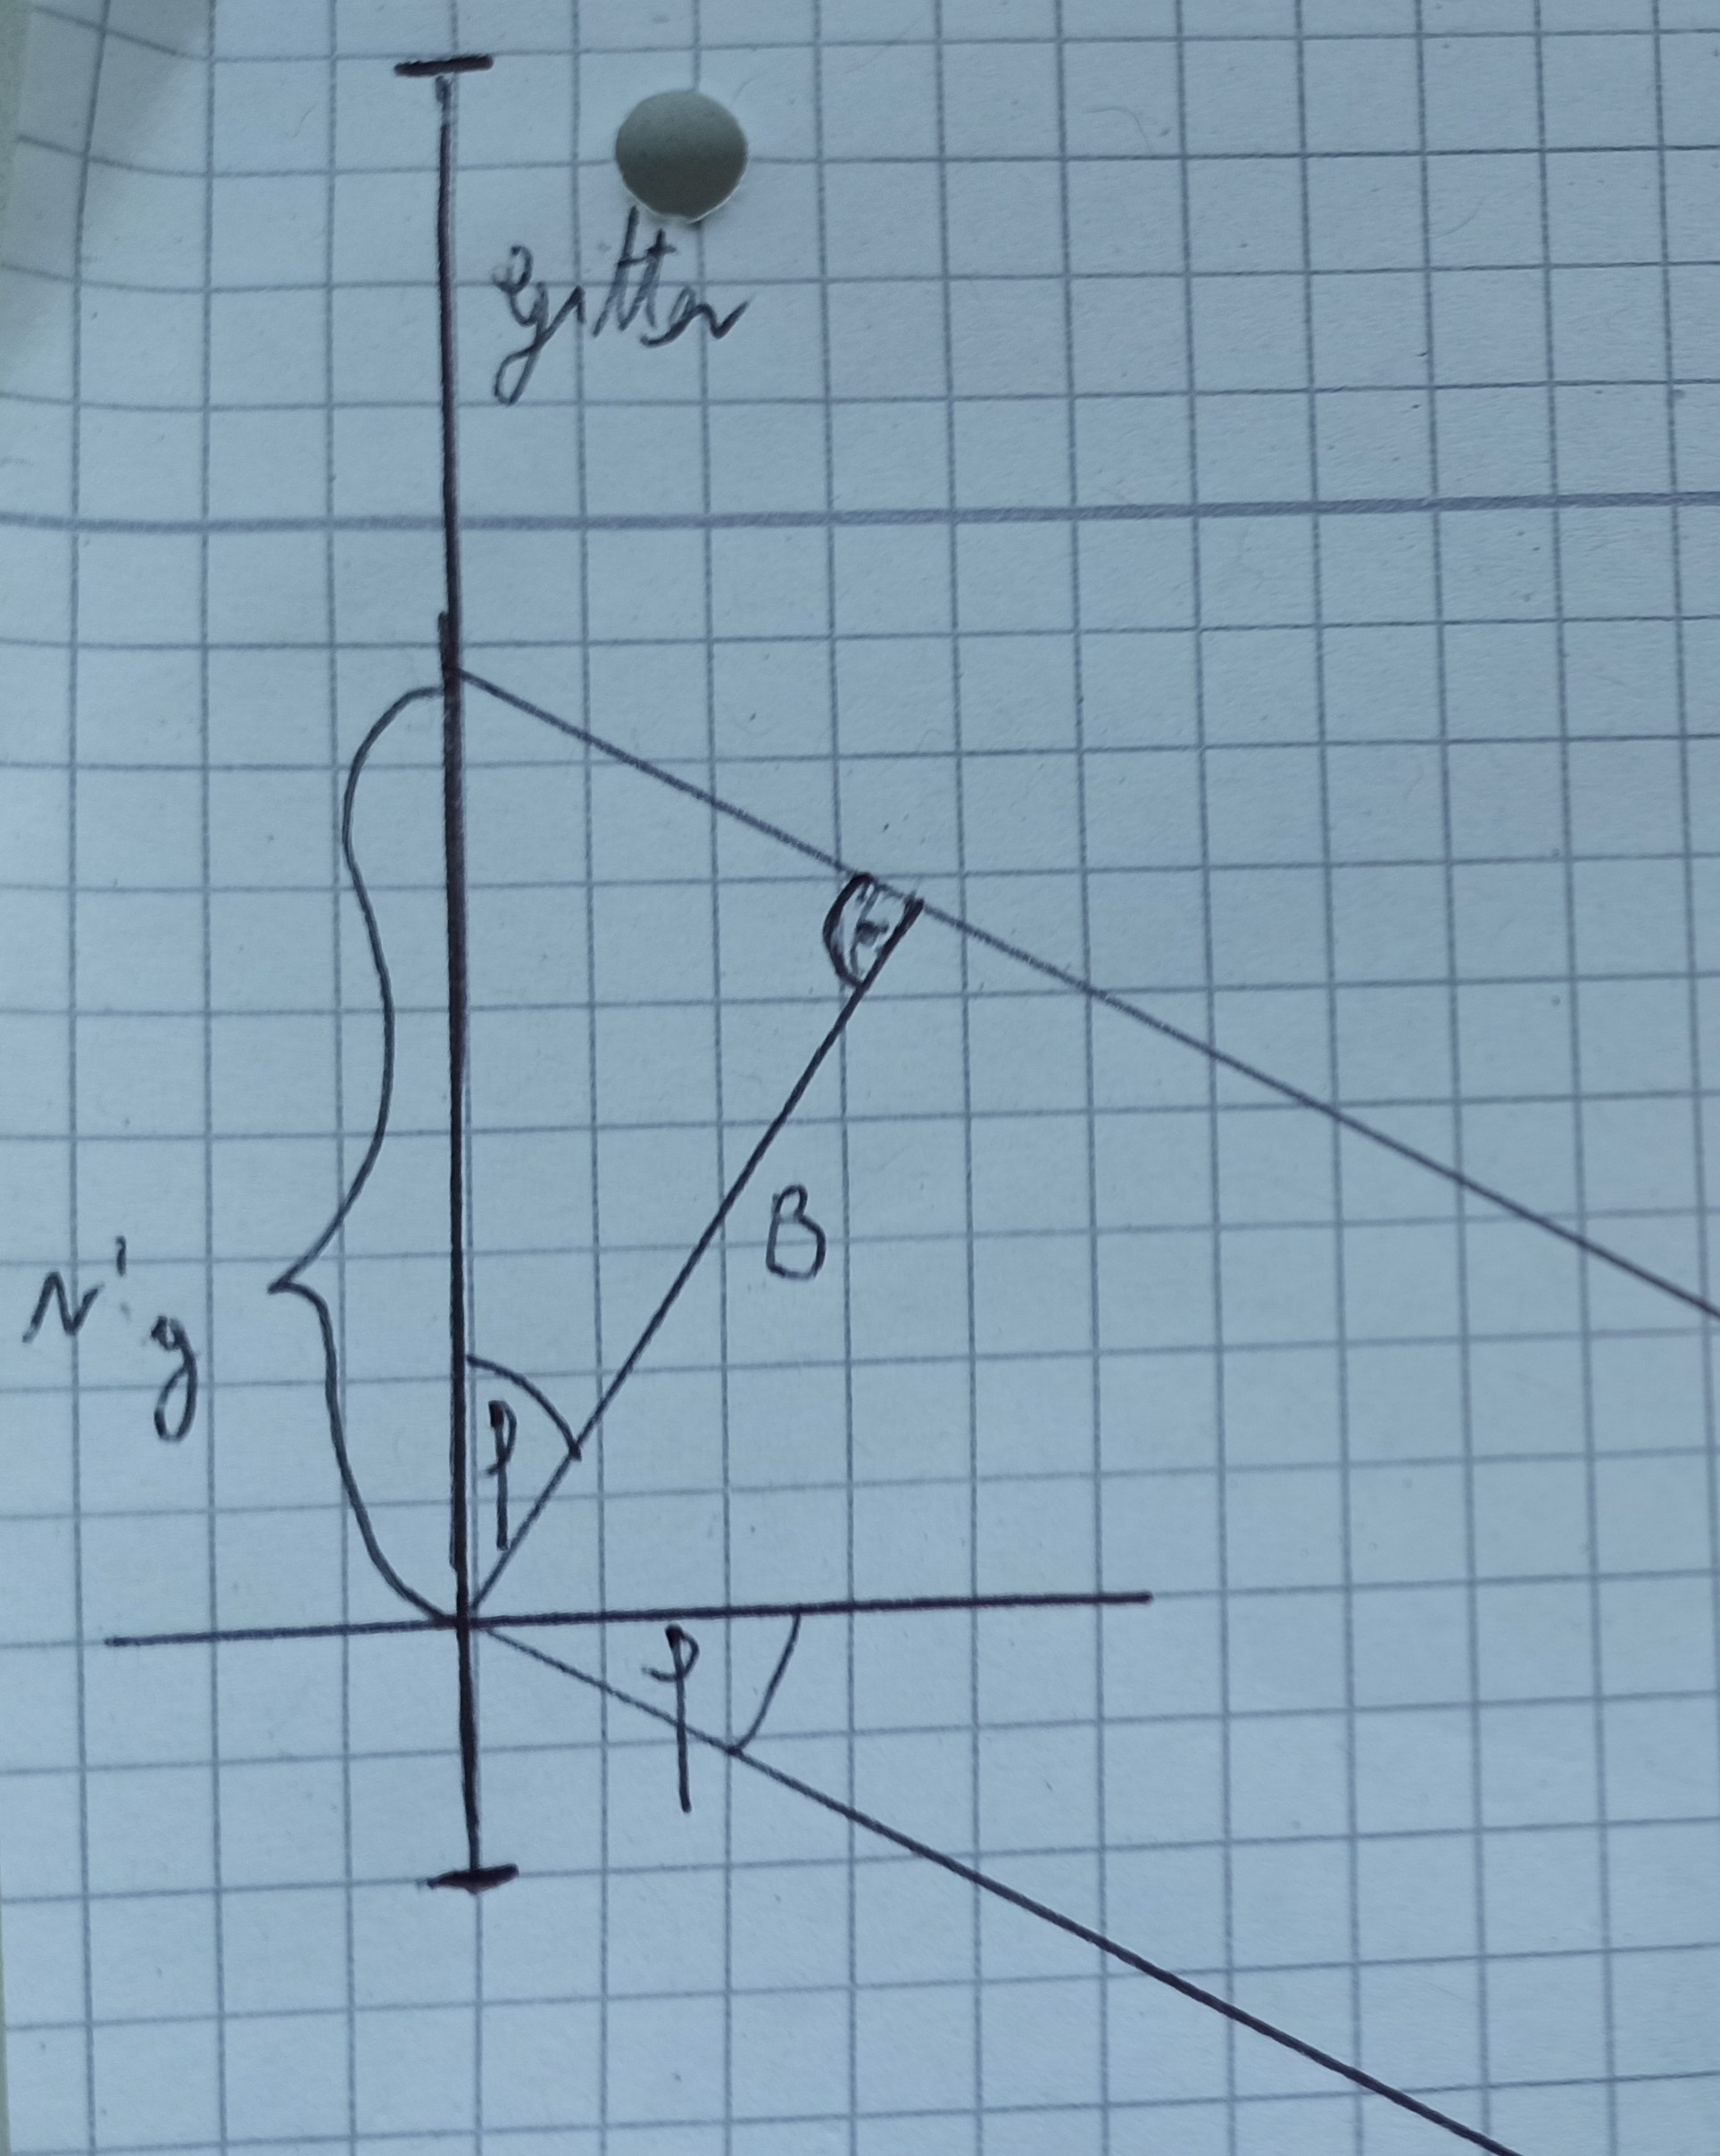
\includegraphics[scale=0.18]{Gitter1}\caption{Schaubild wie der Messspalt einen Teil des Gitters ausschließt}\end{figure}
\begin{equation*}N'\cdot{g}\cdot\sin\varphi=B\end{equation*}
Dadurch verändert sich über die Lage der Minima natürlich auch die Bedingung für die Auflösung. Wenn man diese Bedingung in Gleichung (1) einsetzt und bedenkt, dass man unter diesem Winkel ja immer noch Maxima beobachten will, erhält man
\begin{equation}\frac{\lambda}{\Delta\lambda}=k\,N'=\frac{g\,\sin\varphi}{\lambda}\cdot\frac{B}{g\,\cos\varphi}=\frac{B}{\lambda}\,\tan\varphi\end{equation}
\begin{figure}[H]\centering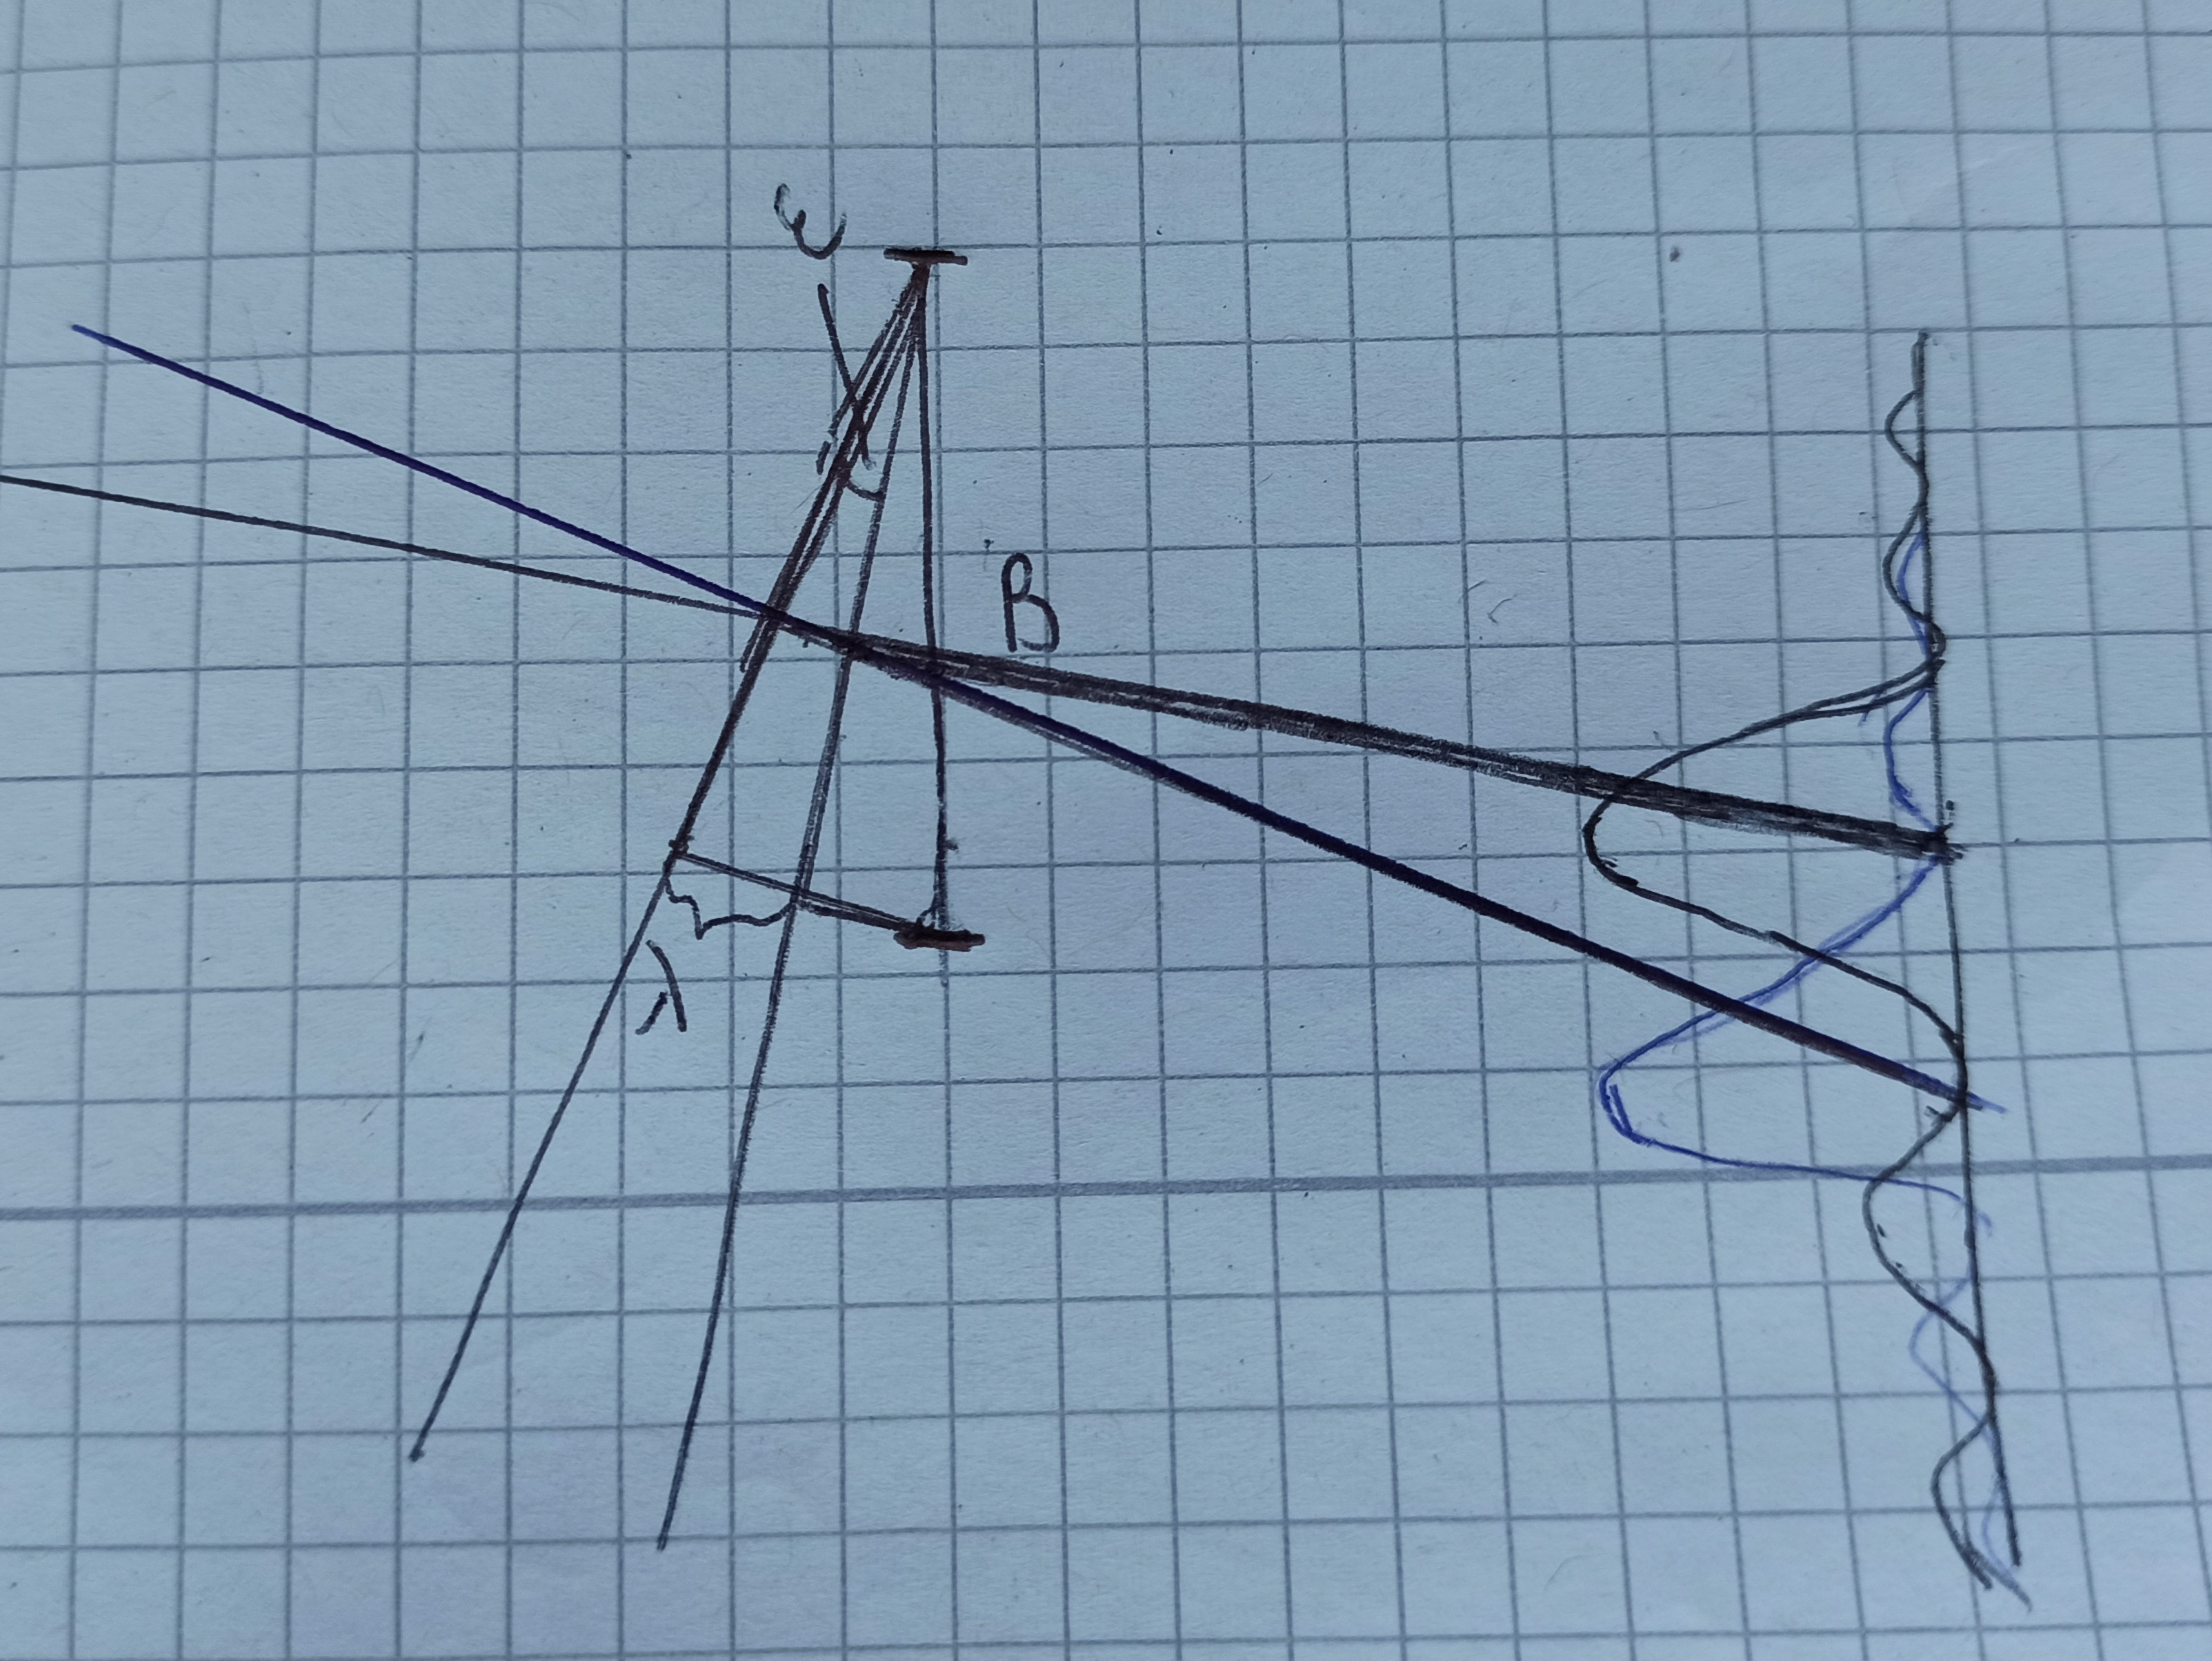
\includegraphics[scale=0.15]{Prisma1}\caption{Wegunterschied beim Auftreffen auf den Messspalt und resultierende Verschiebung der Beugungsmaxima 0. Ordnung}\end{figure}
Im zweiten Teil des Versuchs spalten wir den Lichtstrahl erst durch ein Prisma auf, bevor er durch den Messspalt gebeugt wird. Dadurch verschieben sich die Wellenfronten zu einander. Wir verwenden im Versuch eine Hg-Lampe, deren Spektrum zwei sehr ähnliche Wellenlängen im orangen Bereich besitzt. Der Winkel zwischen den Wellenfronten dieser beiden Farben sei $\epsilon$. Durch diesen Winkel entsteht beim Auftreffen auf den Spalt bereits ein Wegunterschied an den Randpunkten des Spalts. Um die Beugungsmaxima 0. Ordnung der beiden Frequenzen hinter dem Spalt gegeneinander auflösen zu können, muss das Maxima der einen Wellenlänge ins Minima der anderen Fallen. Diese Bedingung lässt sich auch auf Grund des Umstands, das die Wellenlängen fast gleich lang sind, näherungsweise so formulieren, dass der Wegunterschied am Punkt des 0. Beugungsmaximum gerade $\lambda$ sein muss. Da der Wegunterschied beim Auftreffen auf den Spalt $B\cdot\sin\epsilon$ ist, erhalten wir als Minimalbedingung
\begin{equation*}B\cdot\sin\epsilon=\lambda\end{equation*}
oder mit Kleinwinkelnäherung
\begin{equation}\frac{\lambda}{\Delta\lambda}=\frac{B\cdot\epsilon}{\Delta\lambda}\end{equation}

\section{Versuchsdurchführung}
Grundlage unseres Versuches ist, wie oben schon angesprochen, dass wir eine Hg-Lampe verwenden, dessen Spektrum zwei eng benachbarte Wellenlängen besitzt. Wir wollen jeweils bestimmen, bei welcher Spaltbreite die durch Beugung entstandenen Maxima noch von einander trennbar sind. Dadurch möchten wir das Minimale Auflösungsvermögen des Spalts ermitteln, bzw. eigentlich bei einer gewissen Auflösung die minimale Spaltbreite.
In unserem Versuchsaufbau wird der Strahlengang aus der Lampe zunächst durch eine Kollimatorlinse parallel gerichtet. Danach passiert das Licht entweder das Prisma oder das Gitter und danach unseren Messspalt. Um die Beugungsmuster beobachten zu können, schalten wir dem anschließend ein Fernrohr nach, dessen Brennweite auf unendlich gestellt wurde.
Wir starteten unser Experiment, indem wir zunächst den Nullpunkt der Spaltbreite bestimmten. Dazu ermittelten wir den vom Messsystem angezeigten Wert, bei dem ohne Gitter oder Prisma, kein Licht mehr zu beobachten war, bzw. das erste mal wieder Licht gesehen wurde. Beide Zustände bestimmten wir 5 Mal. Folgender Tabelle sind die Messdaten, sowie die erste Auswertung zu entnehmen.
\begin{table}[H]\begin{tabular}{c | c | c | c | c}
Kein Licht&Licht&Mittelwert&stat. Fehler&sys. Fehler\\\hline
0.398&0.374&0.386&0.034&0.005\\\hline
0.398&0.377&0.388&0.03&0.005\\\hline
0.399&0.372&0.386&0.038&0.005\\\hline
0.402&0.387&0.395&0.021&0.005\\\hline
0.403&0.381&0.392&0.031&0.005\end{tabular}\caption{Messdaten zur Kalibrierung der Spaltbreite}\end{table}
Diese Daten pflanzen sich zu $0.389\pm0.031(\text{stat})\pm0.005(\text{sys})\,\text{mm}$ als angezeigte Breite für den geschlossenen Spalt fort.

\section{Auswertung}
Danach stellten wir ein Prisma in den Strahlengang zwischen Spalt und Kollimator und achteten darauf, dass der Strahl den Weg minimaler Ablenkung durch das Prisma nimmt. Bei der Messung gingen wir wie zuvor vor, was wir auch in den nachfolgenden Messungen taten. Wir bestimmten die Spaltbreite, bei der kein Licht, bzw. das erste Mal wieder Licht beobachtet werden konnte.
\begin{table}[H]\begin{tabular}{c | c | c | c | c}
Kein Licht&Licht&Mittelwert&stat. Fehler&sys. Fehler\\\hline
1.529&1.739&1.634&0.297&0.006\\\hline
1.668&1.67&1.669&0.003&0.006\\\hline
1.571&1.674&1.623&0.146&0.006\\\hline
1.562&1.746&1.654&0.26&0.006\\\hline
1.534&1.685&1.61&0.214&0.006\\\hline
\end{tabular}\caption{Messung zum Prisma}\end{table}
Zusammen mit der Kalibrierung ergibt dies eine minimale Spaltbreite von $$B=2.027\pm0.213(\text{stat})\pm0.011(\text{sys})\,\text{mm,}$$
wobei ich zuerst den Mittelwert der Mittelwerte bestimmt und dann die Fehler nach Gauß'schem Fehlerfortpflanzungsgesetz fortgepflanzt habe, und das dann nochmal mit der Kalibrierung verrechnet habe. Da der Winkel zwischen den vermessenen Beugungsmaxima zu bestimmen, der auch dem durch das Prisma verursachten Winkel zwischen den Wellenfronten entspricht, aufgrund ihrer Nähe nicht genau hätte erfolgen können, vermaßen wir den Winkel zwischen dem Beugungsmaximum 0. Ordnung des grünen Lichts ($546.3\,\text{nm}$ Quelle Anleitung) und des Mittelpunkts zwischen den Maxima der beiden orangenen Wellenlängen ($578.2\,\text{nm}$ Quelle Wikipedia). Dieser Winkel beträgt $0.5^\circ$. Wir nehmen nun an, dass der Ablenkwinkel des Prismas linear von der Wellenlänge abhängt. Umgerechnet entspricht das also einem Winkel zwischen den beiden Wellenlängen von $\epsilon=0.0174^\circ$. Daraus lässt sich ein Auflösungsvermögen von $$\lambda/\Delta\lambda=554.48\pm58.27(\text{stat})\pm12.53(\text{sys})$$
berechnen. Die systematischen Fehler wurden als die Hälfte der kleinsten Ableseeinheit zuzüglich 0.5 Promille des Messwertes abgeschätzt. Die kleinste Ableseeinheit war bei der Messung der Spaltbreite $0.01\,\text{mm}$ und bei der Messung des Winkels $0.5/30^\circ$.\newline\newline
Im zweiten Teil des Versuchs ersetzten wir das Prisma durch ein Gitter. Dabei gingen wir methodisch gleich vor. Wir bestimmten wieder die minimale Spaltbreite, bei der die Beugungsmaxima trennbar waren.
\begin{table}[H]\begin{tabular}{c | c | c | c | c}
Kein Licht&Licht&Mittelwert&stat. Fehler&sys. Fehler\\\hline
0.86&1.07&0.965&0.297&0.005\\\hline
1.005&1.05&1.028&0.064&0.006\\\hline
0.9&1.112&1.006&0.3&0.006\\\hline
0.9&1.065&0.983&0.233&0.005\\\hline
0.8&1.05&0.925&0.354&0.005
\end{tabular}\caption{Vermessung der 2. Beugungsordnung}\end{table}
Daraus bestimmt sich die minimale Spaltbreite auf $B=1.370\pm0.270(\text{stat})\pm0.011(\text{sys})\,\text{mm}$. Wir beobachteten die zweite Beugungsordnung unter dem Winkel $\varphi=24.567\pm0.021(\text{sys})\,^\circ$. Damit lässt sich das Auflösungsvermögen auf $\lambda/\Delta\lambda=276.20\pm54.57(\text{stat})\pm30.20(\text{sys})$. Als Wellenlänge wurde hier o.B.d.A die Wellenlänge der kurzwelligeren der beiden orangenen Linien mit $576.96\,\text{nm}$ (laut Wikipedia) verwendet.
\begin{table}[H]\begin{tabular}{c | c | c | c | c}
Kein Licht&Licht&Mittelwert&stat. Fehler&sys. Fehler\\\hline
0.39&0.52&0.455&0.184&0.005\\\hline
0.39&0.49&0.44&0.141&0.005\\\hline
0.43&0.495&0.463&0.092&0.005\\\hline
0.435&0.52&0.478&0.12&0.005\\\hline
0.42&0.49&0.455&0.099&0.005
\end{tabular}\caption{Vermessung der 3. Beugungsordnung}\end{table}
Aus der Messung der 3. Beugungsordnung ergibt sich der minimale Spalt als $B=0.847\pm0.135(\text{stat})\pm0.010(\text{sys})\,\text{mm}$. Mit einem Winkel von $27.933\pm0.022(\text{sys})\,^\circ$ berechnet sich eine Auflösung von $\lambda/\Delta\lambda=258.89\pm41.32(\text{stat})\pm23.37(\text{sys})\,$.
Für die vierte Ordnung
\begin{table}[H]\begin{tabular}{c | c | c | c | c}
Kein Licht&Licht&Mittelwert&stat. Fehler&sys. Fehler\\\hline
0.21&0.258&0.234&0.068&0.005\\\hline
0.215&0.3&0.258&0.12&0.005\\\hline
0.22&0.3&0.26&0.113	&0.005\\\hline
0.23&0.27&0.25&0.057&0.005\\\hline
0.22&0.29&0.255&0.099&0.005
\end{tabular}\caption{Vermessung der vierten Beugungsordnung}\end{table}
ergibt sich eine minimale Breite des Messspalts von $B=0.640\pm0.100(\text{stat})\pm0.010(\text{sys})\,\text{mm}$ und ein Winkel von $31.333\pm0.024(\text{sys})\,^\circ$. Die Auflösung resultiert dann zu $\lambda/\Delta\lambda=264.43\pm41.20(\text{stat})\pm21.89(\text{sys})\,$.

\section{Fazit}
Im Vergleich zur bekannten Auflösung aus $\lambda/\Delta\lambda=576.96\,\text{nm}/2.11\,\text{nm}=273.44$ lässt sich feststellen, dass die Spaltbreite im Versuch beim Gitter, die Auflösung ziemlich gut repräsentiert, während es im Versuch mit dem Prisma doch eine sehr starke Abweichung gibt. Dies kann ein Stück weit mit der Ungenauigkeit der Messtechnik erklärt werden. Das beste Ergebnis erzielte die Messung bei der zweiten Beugungsordnung des Gitters. Ein Grund, weshalb die Messungen höherer Ordnung ein etwas schlechteres Ergebnis brachten, ist wahrscheinlich auch, dass bei größeren Winkeln der Fehler der Kleinwinkelnäherung zunimmt.

















\end{document}